\chapter{Methodology}\label{chap2}
\thispagestyle{plain}
In this chapter an overview of the data used to train the machine learning models, the mathematical principle behind these models and the methods used to asses their accuracy will be presented. 

%This chapter provides a detailed description of the methodology. It is
%sometimes called Experimental Section. Depending on the subject it is a
%``synonym'', e.g., for Theoretical Section, Computational Methods, Model
%Description and Setup, Field Work, and so on. Hence, this chapter contains a
%description of \emph{what has been done} in order to address the scientific
%question raised in the chapter Introduction. However, it does \emph{not} contain
%the results! 


% ==== SECTION 1 ===============================================================
%\section{Experimental Set-up}\label{2sec:1}
%Depending on the topic of the science thesis, this chapter may contain a
%description of the experimental set-up, the field experiment,
%datasets, instruments, measurement procedures, analysis techniques, calibration
%and quality control, and other things. In case of a modeling study it may
%contain the formulation and derivation of model equations, the formulation of
%initial and boundary conditions, the data used to drive and validate the model,
%an overview of the model set-up (e.g., parameter set-up), modifications of the
%``original'' model code, a description of relevant parameterizations,
%a theoretical background needed for the interpretation of model results.


% ==== SECTION 2 ===============================================================
\section{Data Sets}\label{glathida}
The first section gives an overview of the data used in the analysis done in this thesis. The data used to train and analyze the machine learning models are: the Glacier Thickness Database (GlaThiDa), the Randolph Glacier Inventory (RGI), and different digital elevation models (DEMs) which depend on the specific glacier. Depending on the region in fact, some digital elevation models are a better fitted to each glacier, as all of the freely available ones have missing data. ``The best'' digital elevation model for each glacier has been automatically chosen by the Open Global Glacier Model (OGGM). Through most of the analysis SRTM v4 \citep{SRTM} which is a 90m grid resolution DEM has been used. Other DEM have been used to link the GlaThiDa with RGI (see section \ref{GlaRGI})

\subsection{Glacier Thickness Database}
The Glacier Thickness Database \citep{GlaThiDa2014} is the most comprehensive set of data including available ice thickness measurements from glaciers and ice caps all around the globe. The database is composed of three different tables. The first one contains an overview of the database, the second one thickness data averaged over surface elevation bands, and the third one, the one used in this thesis, contains the actual in-situ point-wise ice thickness observations. 

The third table of the database contains ice thickness observations deriving from a vast number of different campaigns led by different research groups worldwide. The GlaThiDa is an inventory attempting to gather all these different observations into one single database.
 
There are two main way for the measurements to be gathered: glacier exploration, i.e. walking on the glacier, and airborne measurements which are the majority of the entries in the GlaThiDa. Different measuring methods and instruments were used to obtain the ice thickness values. The most widely used method is Ground Penetrating Radar (GPR), used in both airborne and terrestrial explorations, which uses electromagnetic waves to obtain information about subsurface characteristics and structures. It has a relatively easy application and limited process required for data interpolation but has the disadvantage of decreasing resolution at the low frequencies \citep{van2012} necessary to obtain ice thickness measurements. Other methods are seismic methods, based on the traveling velocity of elastic waves through different materials, and direct drilling.

Each of the observation available in the third table is accompanied by relevant data about the observation itself. Among the others these data are: longitude and latitude coordinates of the point-observation, a unique point-id which is used to identify the observation uniquely across the database, the name of the glacier where the observations was taken, the name of the country in which the glacier is located, the date of the survey, the survey method, and the thickness uncertainty. Some of these data however are not always filled in for each of the measurements as it is often the case for the glacier name and the uncertainties. For the latter the authors of the database suggest to consider the uncertainties of the individual methods used to obtain the observations,  as a minimum estimate for the measure uncertainties. The problem of linking each measurement with its glacier can instead be addressed using the Randolph Glacier Inventory (RGI, see section \ref{rgi}), which provides the shape and its coordinates for every glacier worldwide. This, together with the GPS coordinates of the GlaThiDa, allow to assign each measurement to the glacier it belongs, if the measurements coordinates lie inside any of the glaciers present in the RGI, which is not always the case. 

The first GlaThiDa was released in 2014. In 2016 a second version 2.0 and its correction 2.1 were released, and in 2019 version 3.0 and 3.01 were finally released. All the analysis in this work have been done using version 2.1 as version 3.0 was released after most of the analysis were already done. According to the GlaThiDa \href{https://github.com/ezwelty/glathida/blob/master/CHANGELOG.md}{change-log} however most of the changes have been done to the structure of the data base. There were however, some measurements additions to the database. The addition of some measurements for some glaciers in Switzerland in particular could be relevant for this thesis, given that most of the analysis done in this work has been conducted over the alpine glaciers. 
%Use subsections to structure your thesis. The first and second component of the
%momentum equation is shown in equation (\ref{2equ:1}) and (\ref{2equ:2}),
%respectively. Together with (\ref{2equ:3}) they form the set of shallow-water
%equations implemented in a numerical model.

\subsection{Randolph Glacier Inventory}\label{rgi}
The Randolph Glacier Inventory (RGI) \citep{RGI2014} is a global database of outlines of glaciers and ice caps. The inventory has been compiled from satellite imagery collected since 1999 onward. Most of the outlines don't express a specific picture in time of the glacier, but are a compound of different images of each glacier due to images obstructions such as cloud covers or satellite orbits. The first version of this inventory was released in 2012 and the latest version, RGI Version 6.0 was released in 2017. In this latest release the database comprises more than 220,000 glacier outlines which are divided in 19, regions covering all areas in the world with glaciers. This is the version used for all the analysis in this thesis. 


\subsection{Linking GlaThiDa and RGI}\label{GlaRGI}
The GlaThiDa comes with a table containing the thickness measurements observations. This table contains the thickness value of the observation, its latitude and longitude, and other variables such as the date of the observation, the name of the glacier, the thickness uncertainty and others. Aside from GPS coordinates and thickness value, some fields like, the name of the glacier and the thickness uncertainty, are often left empty. This creates the problem of having to link each observation with a glacier in the RGI database. To do so a script has been created which determines whether an observation is located inside a glacier outline: the RGI database comes with closed outlines of the glaciers in geographic coordinates referenced to the WSG84 (also known as ESPG:4326) as shape-files. The python library \href{https://github.com/Toblerity/Shapely}{shapely} has been used to transform the observations latitude and longitude to the WSG84 projection system, and to check whether each of these point was lying inside the glacier outlines (including the boundaries of the outline).

\begin{figure}\label{fig:thickness-pt} 
	\centering 
	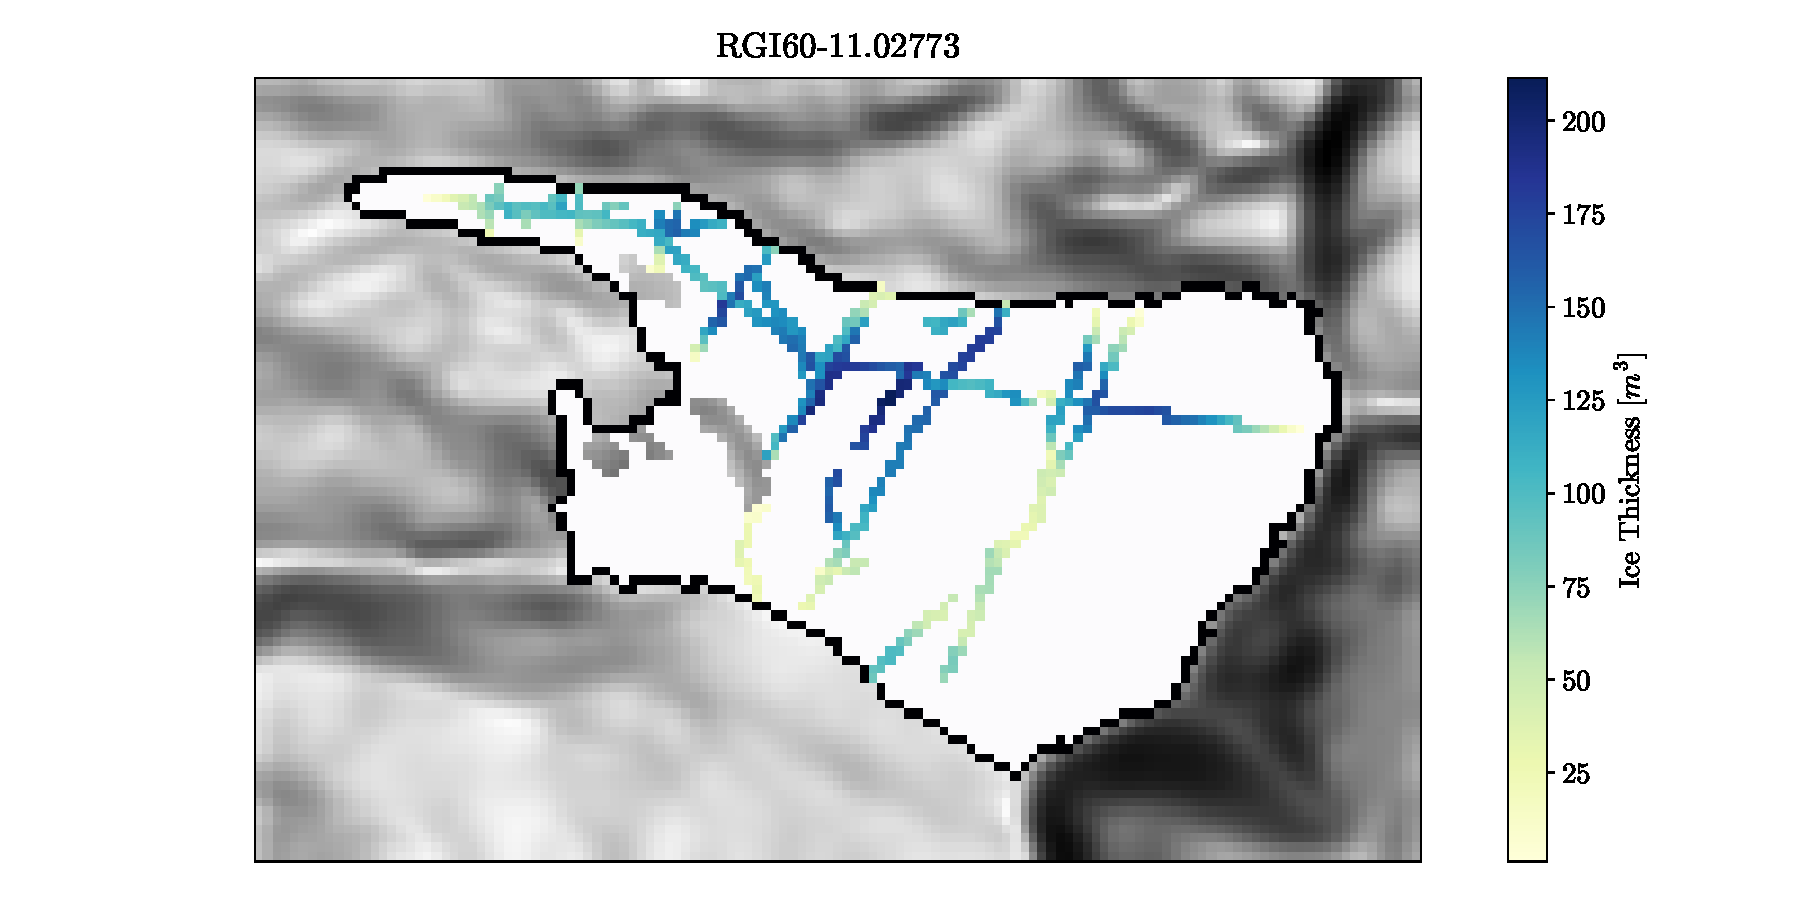
\includegraphics[width=1.0\textwidth]{./figures/glathida_thick_map.pdf}
	\caption{Map of glacier RGI60-11.02773 with ice thickness observations after processing the glacier with OGGM: ice thickness observations are the average ice thickness for all observations inside a grid cell.}
\end{figure}

\subsection{Some statistics about GlaThiDa}\label{glathida-stats}
After linking the two databases it is interesting to learn about some statistics of the GlaThiDa. In order to create these statistics the Open Global Glacier Model (OGGM) \citep{OGGM2019}, \href{https://github.com/OGGM/oggm}{Open Source Code}) has been used to add a digital elevation model to the glaciers in the RGI with thickness entries in the GlaThiDa (see \ref{GlaRGI}).

\subsubsection{Glaciers distribution and types}
There are 820370 entries (ice thickness observation points) in the GlaThiDa version 2.1. After assigning each of them to one of the 215,547 RGI glaciers, 771 of those glaciers have resulted to have thickness observations associated with them. This is 0.36\% of all the glaciers in th RGI. Out of the 820370 initial entries 27882, 3.4\% of them, resulted outside any glacier outlines defined in the RGI. Some reason for this could be: a slightly wrong GPS coordinate reported in the GlaThiDa, observations taken outside of the glacier by mistake or intentionally, to make sure that all the glacier was covered, a different shape of the glacier at the moment when the observation was taken, compared to the moment when the RGI was compiled, a wrong assessment of the glacier shape in the RGI.
\begin{figure}[tp]\label{glathidamap} 
	\centering 
	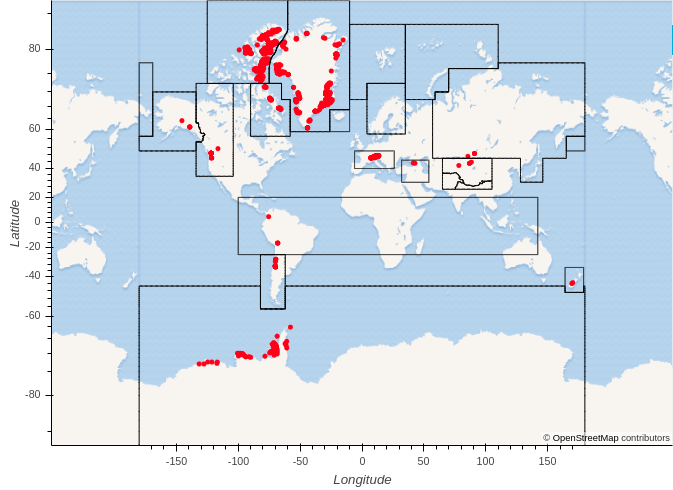
\includegraphics[width=0.93\textwidth]{./figures/GlaThiDa_map.png}
	\caption{Global map of the distribution of glaciers with thickness observations entries in the GlaThiDa database version 2.1. Black outlines are the RGI regions.}
\end{figure}

Most of the glaciers with thickness observation are in the Greenland Periphery region and in the Artic Canada North region (see Fig. \ref{fig:glareg}). If we compare the glaciers with measurements with the number of glaciers present in each specific region however, we see that Arctic Canada North is the best represented region with around 5\% of the glaciers having at least one thickness measurement point. The region with most glaciers in the RGI, Central Asia, has a very low number of glaciers represented in the GlaThiDa database. This is probably due to the difficulties encountered when trying to get measurements for glaciers at such high altitudes as those reached in the Himalaya and the fact that no airborne campaigns have been led in this area.


\begin{figure}[!tp]
	\centering		  
	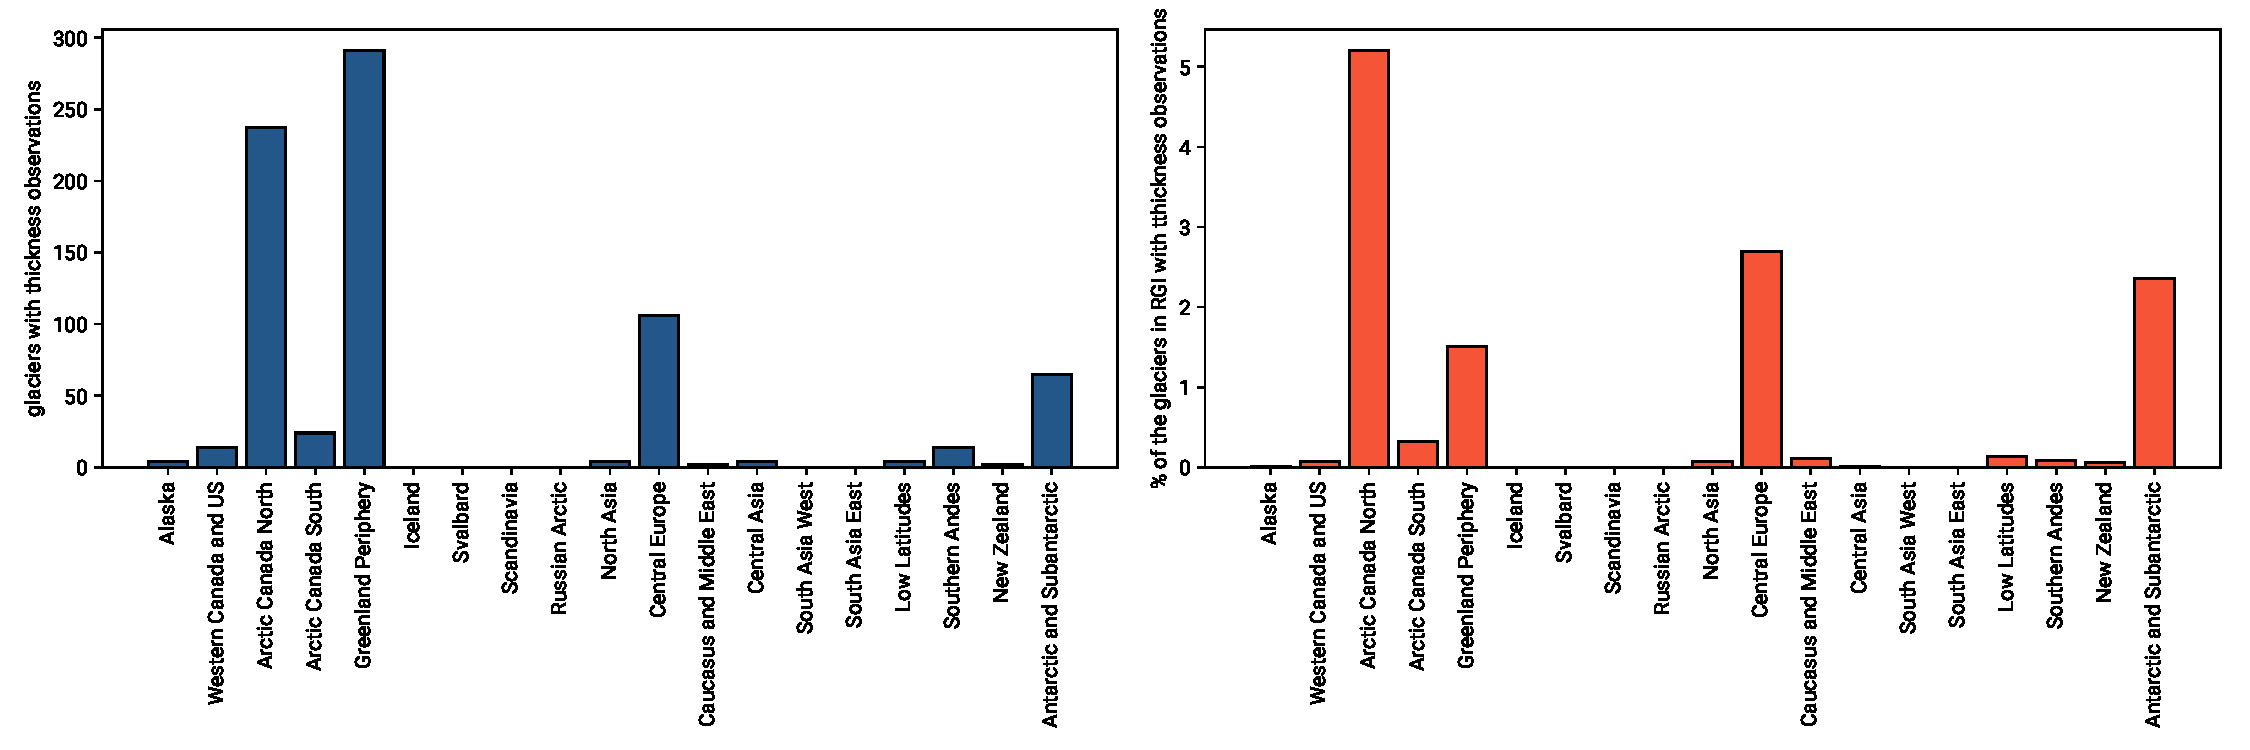
\includegraphics[width=1.\textwidth]{figures/Observations_per_region.pdf}
	\caption{On the left side the number of glaciers in the RGI with thickness observations in the GlaThiDa are shown per RGI region. On the right side the percentage of glaciers for each region with thickness observations is shown instead.}
	\label{fig:glareg}
\end{figure}

More than two third of the RGI entities with GlaThiDa measurements are glaciers, while the rest are ice caps. Land terminating glaciers and ice caps are the vast majority.

\subsubsection{Measurements Distribution per Glacier}
Not all the glaciers with measurements are perfectly covered over the whole glacier area. In fact around 42\% of the glaciers have less than 100 thickness observations. Given that some glaciers can extend for over $100 km^2$, it’s clear that some of them are very poorly covered.
\begin{figure}[!bp]
	\centering		  
	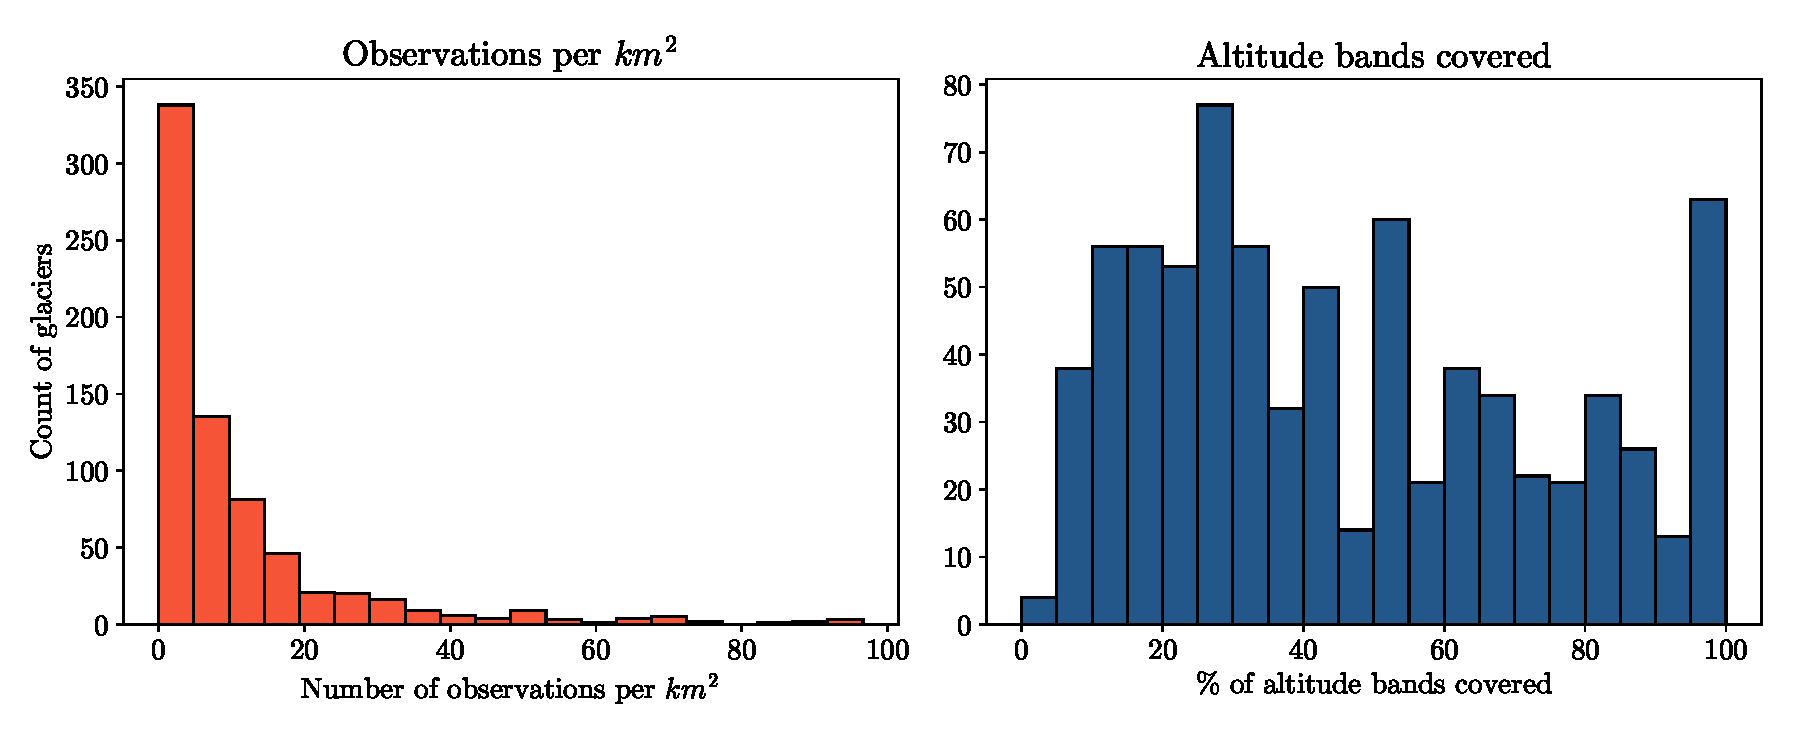
\includegraphics[width=1.\textwidth]{figures/Observations_per_skm.pdf}
	\caption{On the Left: distribution of glaciers with less than 100 observations per squared kilometer; there is a great number of glaciers with less than 20 thickness observations per squared kilometer. On the right: distribution of glaciers according to the percentage of their 100$m$ altitude bands covered.}
	\label{fig:glaobs}
\end{figure}

More than 91\% of all the glaciers have less than 100 thickness measurements per squared kilometer (see Fig. \ref{fig:glaobs}). Almost 44\% of all the glaciers with thickness observations have less than 5 observations per squared kilometer.

OGGM was used to generate a gridded map of each glacier represented in the GlaThiDa. With this map one can divide each glacier in $100m$ altitude bands to check how many of those bands contain at least one thickness measurement.
Almost half of the glaciers have observations in at least half of the 100m altitude bands (see Fig. \ref{fig:glaobs}). Glaciers with few observations but well distributed over their length can be very useful to understand glacier thickness patterns and for model validation.

\subsubsection{Survey Year}\label{survey-year}
Measurements were taken between 1977 and 2015, but most of them after 2005 (see Fig. \ref{fig:glayears}). The spread in the dates of the campaigns to take the observations could potentially create problems when trying to compare glaciers with each other to find similar patterns, but also when using the data for model validation.
Most glacier models in fact, use digital elevation models to setup the model run. Any digital elevation model is compiled with data available at the time of its construction. The time difference between the date of data assimilation for the digital elevation model, and the date of the survey for the thickness observation, could be in the order of several years. This would create an error when validating the model.
\begin{figure}[!tp]
	\centering		  
	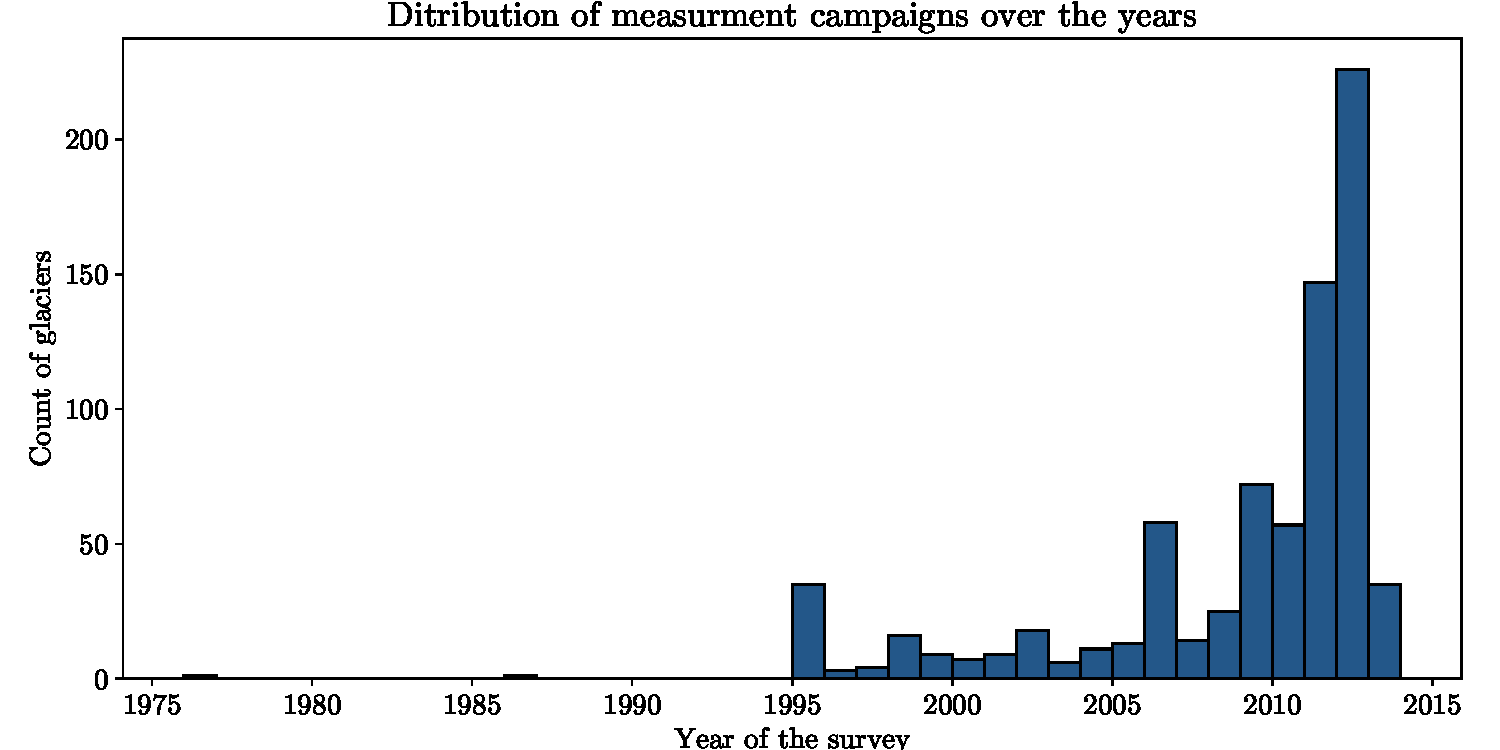
\includegraphics[width=1.\textwidth]{figures/Observations_per_year.pdf}
	\caption{Distribution of glaciers with observations in the GlaThiDa according to the year when the measurements for each glacier were taken.}
	\label{fig:glayears}
\end{figure}


\section{Machine Learning Algorithms}\label{ML}
Machine learning is a mathematical method which enables computers to perform a specific task without giving it specific instructions on how to do it. This is achieved using algorithms which build a model from a sample of data usually called the ``training data''. The algorithm then uses these data in an iterative process, called the training process, to improve its performance at solving the requested task. After the iteration process is finished the model is trained and we can use it to solve our task. 

The idea behind machine learning is to emulate the learning process of a human-being in order to make predictions about new data. If for example one wanted to teach a kid how to recognize a cat, the simpler approach would be to show it cats or pictures of them, instead of trying to explain to it the key characteristics of cats. In a similar way machine learning algorithms are used to solve tasks without giving them instructions about how to solve them (explaining the key characteristics), but rather by feeding them on examples.

The branch of machine learning used in this thesis is called ``supervised learning'' which builds models learning from data containing the input variables (often referred to as features) and the desired output values, often referred to as labels.
The machine learning algorithm is then used to find the target function $f$ which better maps the input vector $X$ to an output one $Y$.
\begin{equation}
Y = f(X)
\end{equation}
The way this function is computed by the algorithm depends on the specific one chosen to achieve the desired result.

In this thesis three different machine learning algorithms have been used to train models, which estimate the ice thickness of glaciers using the GlaThiDa database as the desired output ($Y$), and use digital elevation models and some basic physical assumptions as the input values ($X$), to estimate the ice thickness distribution of the glacier.

The three algorithms used are:
\begin{itemize}
	\item Linear Regression (LR)
	\item Random Forest Regression (RFR)
	\item Support Vector Regression (SVR)
\end{itemize}

The linear regression is one of the simplest machine learning models, but is has been chosen because it can be used as a reference point for the performances of the other algorithms.

Random forest regression has been chosen to see how a method based on decision tree classification, (see section \ref{random-forest}) can perform on a problem mostly driven by physical dynamics, such as that of the prediction of glaciers ice thickness. 

Support vector regression has been chosen because it is on the other end of the spectrum compared to linear regression, as it is one of the most sophisticated machine learning algorithms. The drawback of using it is that is also one of the most computational expensive algorithms. 

The algorithms have been applied to the data using the python package \href{https://scikit-learn.org/}{scikit learn} \citep{scikit}.
%The way the algorithm achieves this without instructions from the programmer is with an iterative process which uses the training data to make a first prediction, compare the prediction with the the desired output value, 
\subsection{Linear Regression}\label{linearregr}
Linear Regression is probably one of the simplest machine learning algorithms and also one of the most used (even though many people probably don't know it is considered a machine learning algorithm).

Given a set of input data $\bm{X} = \{x_{i1},\ldots ,x_{ip}\}_{i=1}^{n}$ and a corresponding output $\mathbf{y} = \{y_{1},\ldots ,y_{n}\}$, the algorithm finds the best set of $\bm{\beta} = \{\beta_{1},\ldots ,\beta_{p}\}$, and $\varepsilon$, a scalar often referred to as the intercept, such that:
\begin{equation}\label{eq:linear}
\mathbf {y} = \varepsilon + \bm{\beta}\bm{X}
\end{equation}
In order to find $\varepsilon$ and $\bm{\beta}$ which best predict the desired $\mathbf {y}$, one of the most common approaches is to minimize the loss function
\begin{equation}
\frac{1}{n}\sum_{1}^{n}(y_i-y^*_i)^2
\end{equation}
where $y_i$ is the value of the $i$-th prediction generated by the model and $y^*_i$ is the corresponding value the model is trying to predict.

This algorithm is clearly only useful for cases when the output variables linearly depend on the input ones. This is however often not the case thus requiring most sophisticated models to compute the desired output values. It can be helpful however to compare this method to the more sophisticated ones to have a basic reference on their performances.

\subsection{Random Forest}\label{random-forest}
\begin{figure}[!tp]
	\centering		  
	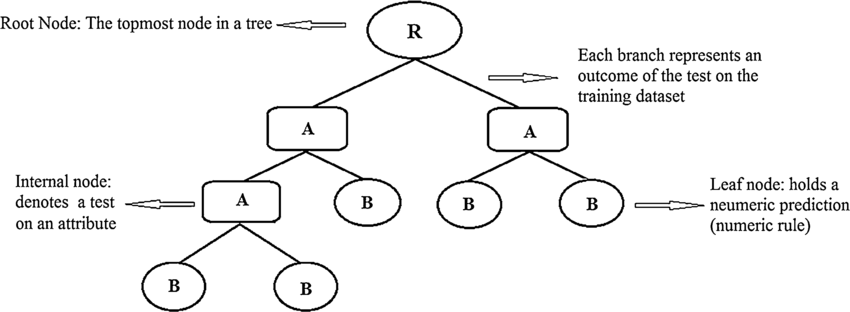
\includegraphics[width=1.\textwidth]{figures/decision_tree.png}
	\caption{Representation of a decision tree model. The tree is pictured upside-down with the root on the top and the branches and leaves on the bottom.}
	\label{fig:tree}
\end{figure}
Random Forest is an algorithm which uses ensemble learning to extend and improve the performances of decision trees algorithm. The method was first proposed by \citet{RandomHo1995}. 

A decision tree is an algorithm used to predict the desired value from a set of data. It works by splitting the data-set at so called nodes, into a number of branches by imposing conditions on a feature. Every split leads to two different subsets of the data-set, which can each be split further, to better achieve the desired outcome. The top part of the tree is called the root and is the first node of the tree, and the bottom parts, which contain the numerical predictions are called the leaves (see Fig. \ref{fig:tree}).

In order to choose how to split the data on each node the algorithm calculates the sum of the squared residual for splitting the data-set on a particular condition and chooses the condition which minimizes this sum. Let $\bm{X} = \{x_{i1},\ldots ,x_{ip}\}_{i=1}^{n}$ be the $n$ input values, $p$ the different attributes (features) in our data-set, and $\mathbf{y} = \{y_{1},\ldots ,y_{n}\}$ the output values (the values we want to predict). Let assume for simplicity that we are splitting the data based on a condition on the first attribute. The first node in the tree divides the data-set into two subsets $S_1$ with $l$ data points and $S_2$ with $n-l$ data points. The algorithm finds the subsets $S_1$ and $S_2$ which minimize:
\begin{equation}\label{eq:trees}
\sum_{i \in S_1}(\overline{y_1}-y_i)^2 + \sum_{j \in S_2}(\overline{y_2}-y_j)^2
\end{equation}
where  $\overline{y_1} = \frac{1}{l}\sum_{i \in S_1}y_i$ and $\overline{y_2} = \frac{1}{n-l}\sum_{j \in S_2}y_j$. It does so by actually computing Eq. \ref{eq:trees} for all the possible $S_1$ and $S_2$. The method can then be repeated to create further branches and a deeper tree. In order to choose which feature to use as a condition for the split, $S_1$ and $S_2$ are determined for each of the $p$ features in the data-set and the feature chosen is the one achieving the lowest value for Eq. \ref{eq:trees}. The algorithm usually stops when the minimum arbitrary number of observations for each subset is reached or when the maximum desired depth of the tree is reached. The depth of the tree is defined as the maximum length of the longest path form the root to the leafs. The predictions at each leaf are then determined by $\overline{y_1}$ and $\overline{y_2}$.

The method described above also has the advantage of giving a simple way of computing which of the $p$ features are the most important in determining the outcome of the prediction (see section \ref{featuresimp}). This value, known as features importance, can be calculated as the decrease in the node variance weighted by the probability of reaching that node. This probability is determined by the number of samples reaching the node, divided by the total number of samples. The higher the value the more important the feature. 

The problem with decision trees is that they can be accurate at predicting data used to train them, but they usually are inaccurate for predictions of new data (\cite{hastie01statisticallearning}).
To solve this problem the random forest algorithm relays on an ensemble of decision trees to make the predictions. Each tree in the ensemble (forest) is constructed using the same number of input values $n$, but randomly selecting the input values with replacement: each input value can be chosen more then once to be part of the sample constructing the three, leaving out some of the other input values from this sample. In addition to this, each tree is only limited to a subset of features to choose from to split the data at each node. After each tree is trained the prediction is made by averaging the predictions from all the trees in the forest. Additionally an estimate of the uncertainty of the prediction can be calculated from the standard deviation of the predictions from all the trees.



\subsection{Support Vector Regression}\label{support-vector}
Support Vector Regression (SVR) was first presented as the regression extension of the support vector machine algorithm (SVM) by \citet{SVR1997}. Support vector machine is a supervised machine learning algorithm for classification (i.e. the desired output has binary values) first proposed by \citet{SVM1964}.

Let assume a training data-set of $n$ points ${({\mathbf {x}}_{1},y_{1}),\ldots ,({\mathbf {x}}_{n},y_{n}),}$, where $y_{i}$ are either $1$ or -$1$, each indicating a different class, the value we want to predict, for the points ${\mathbf {x}}_{i}$. Each ${\mathbf {x}_{i}}$ is a $p$-dimensional real vector. We want to find the decision boundary that divides the group of points $\mathbf {x}_{i}$ for which $y_{i}=1$ from the group of those for which $y_{i}=-1$. This boundary is defined in such a way that the distance between the hyperplane and the closest ${\mathbf {x}}_{i}$ from either group is maximized.
An hyperplane is defined as the points ${\mathbf {x}}$ satisfying 
\begin{equation}\label{eq:svm}
\mathbf {w}\cdot \mathbf {x}-b=0
\end{equation}

where $\mathbf {w}$ is the normal vector to the plane. $b$ determines the offset of the hyperplane from the origin.

If the training data were linearly separable two parallel hyperplanes must exist separating the two classes of data points such that the distance between the two is maximized. The equations for these planes are respectively:

\begin{align}
\label{eq:planes1}
	\begin{split}
	\mathbf {w}\cdot \mathbf {x}-b = 1, \\
	\mathbf {w}\cdot \mathbf {x}-b = -1
	\end{split}
\end{align}

The distance between the two hyperplanes would determine the margin between the two groups. If no data points would lie inside this margin this would be called a hard margin. The data points ${\mathbf {x}}_{i}$ lying nearest to these two hyperplanes are called the support vectors. The hyperplane lying exactly in the middle of the two is called decision boundary. This hyperplane separates the two groups of data. Should one want to label a new data point not used to train the model, this point would be classified depending on which side of the decision boundary it would lie on.

\begin{figure}[!tp]
	\centering		  
	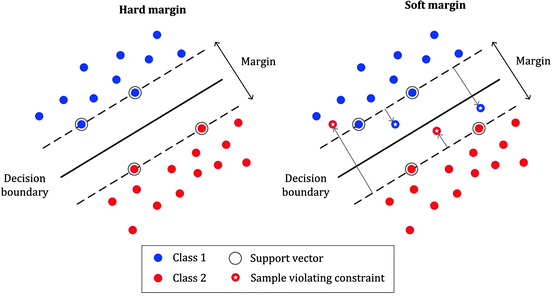
\includegraphics[width=1.\textwidth]{figures/SVM.png}
	\caption{Representation of support vector machine in a 2-dimensional space. On the left a model is trained with the creation of an hard-margin which correctly classifies each sample in the training data-set. On the right a soft-margin is selected which allows a number of miss-classified points to lie inside the margin.}
	\label{fig:svm}
\end{figure}

The distance between the two plains is ${\frac {2}{\|{\mathbf {w}}\|}}$. In order to maximize this distance we then need to minimize $\|{\mathbf {w}}\|$, with the constrain

\begin{equation}\label{eq:svmconstrain}
y_{i}({\mathbf {w}}\cdot {\mathbf {x}}_{i}-b)\geq 1
\end{equation}
for all $i=1,\ldots ,n$ given by the fact that each point must lie outside the margin (see Eq. \ref{eq:svrconstrain}).

This algorithm works well for linearly separable data-sets. However should the data be non linearly separable, or should outliers or miss-classifications be included in the data-set, as in most real world cases, one would instead choose a so called ``soft-margin'', which would work exactly like the hard margin but with allowance for a number of miss-classified data points, data points lying inside the margin. (see Fig. \ref{fig:svm})

To extend this concept for a regression case, i.e. a case where the output values $y_{i}$ are continuous, we can use the same concept, but with the objective of finding a function $f(x)$ which deviates from each $y_{i}$ by a value not greater than $\varepsilon$ and is as flat as possible.

\begin{equation}\label{eq:svr}
f(x) = \mathbf {w}\cdot \mathbf {x}-b
\end{equation}

This would mean to minimize $\|{\mathbf {w}}\|$ subject to the constrain:

\begin{equation}\label{eq:svrconstrain}
|y_{i} - {\mathbf {w}}\cdot {\mathbf {x}}_{i}+b|\leq \varepsilon
\end{equation}
for all $i=1,\ldots ,n$.

To extend the algorithm to non linear cases SVM and SVR apply the so called ``kernel trick''. The algorithm is applied in a transformed higher dimensional space. The resulting boundary hyperplane is linear in the transformed space but might be non linear in the original space.

There are different ways, called kernels, to transform the space to a higher dimensional one. Some of the most common ones, and the ones available in the package \href{https://scikit-learn.org/}{scikit learn} used for the analysis in this thesis, are:
\begin{itemize}
	\item Polynomial
	\item Radial Basis Function
	\item Sigmoid
\end{itemize} 

The one chosen for the analysis in this thesis is the Radial Basis Function kernel (rbf) which transforms the space in this way:
\begin{equation}\label{eq:rbf}
k({\mathbf {x_{i}}},{\mathbf {x_{j}}})=\exp(-\gamma \|\mathbf {x_{i}}-\mathbf {x_{j}}\|^{2})
\end{equation}
for $\gamma >0$.
The kernel basically adds dimensions which are dependent on the distance between the data points. Points with higher distances are less influenced by each other because of the exponential decay which relates the distances.

The kernel trick is what makes support vector regression so powerful because it allows the algorithm to learn from non linear relationship between the data.

\begin{figure}[!tp]
	\centering		  
	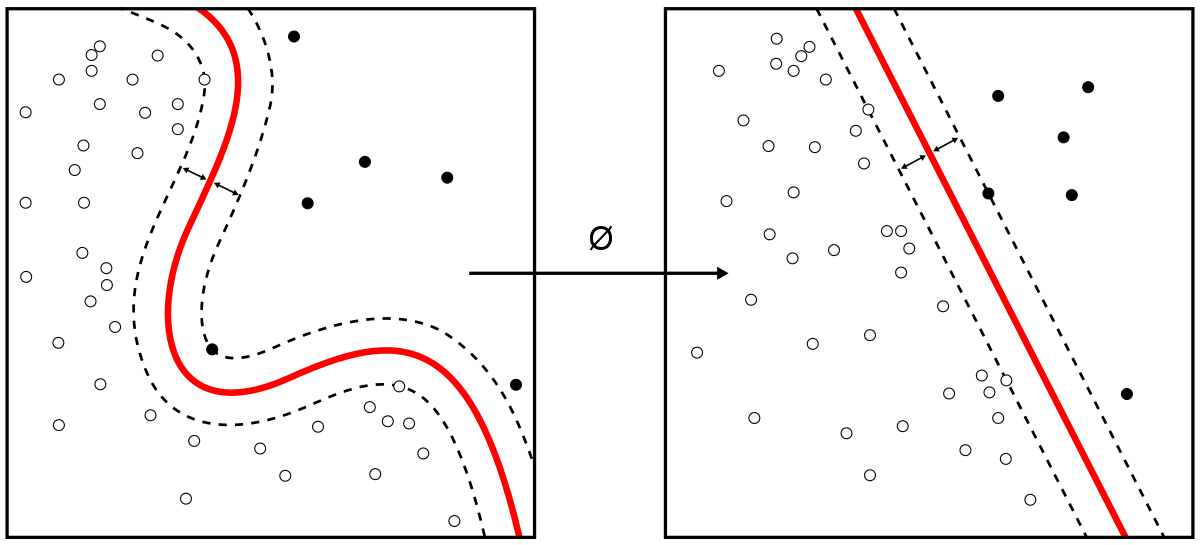
\includegraphics[width=1.\textwidth]{figures/kernel_trick.png}
	\caption{Representation of the kernel trick: the initial 2-dimensional space on the left gets transformed into a 3-dimensional one on the right by the kernel function. An hyperplane can be fitted in the new 3-dimensional space to correctly separate the data with a linear decision boundary.}
	\label{fig:kernel}
\end{figure}


\section{Training method}\label{training}
In order to train the model it is necessary to feed the chosen machine learning algorithm a training data-set. One could simply take all the data from the set and feed them to the algorithm for training. The trained model would then be able to make predictions on a new set of data for which we are lacking labels (the desired output). In the specific case of this thesis, one could take the input parameters chosen to train the model with, from glaciers for which we are lacking ice thickness measurements, and predict the thickness for those glaciers using the trained model. Even more simplistically one could obtain the ice thickness distribution for glaciers where we do have thickness measurements, if those measurements didn't cover the whole glacier surface. In this way we could extrapolate the thickness distribution of the glacier by running the model.

The problem with using all the labeled data available for training however, is the risk of over-fitting the model and the fact that there is no way of assessing the model performances for glaciers without thickness measurements available.
Over-fitting in machine learning means to train a model which is very good at labeling data which were used for training the model, but not able to generalize the results and make predictions about new data. This would lead to a model which is very capable of predicting ice thicknesses for data points which were fed to the algorithm to train it, but wouldn't be able to make correct predictions for data outside the ones used for the training process. 

In order to avoid over-fitting and to be able to have data to assess the performance of the trained model, in a first stage only part of the available data from the GlaThiDa database were fed to the algorithms to train the models. In particular 75\% of the data were used to train the model and the resulting 25\% to asses the performance on new data. This process was achieved with a function available form the python package \href{https://scikit-learn.org/}{scikit learn} which shuffles the data and then randomly picks the data points used for training. The function actually uses a pseudo-random generator to split the data into training and testing samples. It is then possible to always reproduce the same sub-sets of training and testing. This process was then repeated 20 times to be able to compare the model performances subject to training with different sub-sets of data. This should improve the ability of generalization for the trained model, and hence reduce over-fitting. \citep{crossval1995}.

\section{Scoring method}\label{scoring}
Once the model is trained with the training subset of data as described in section \ref{training}, it is important to choose a way to assess the performance of the model. To do this the score method from \href{https://scikit-learn.org/}{scikit learn} has been used on all the models. Let assume the testing input data to consist of $n$ points. Let $y_i$ be the $i$-th prediction done by the model for the $\mathbf{x_i}$ input value of this $n$ points. Let $y^*_i$ be the $i$-th ``true'' label for the $\mathbf{x_i}$ input value, and $\overline{y^*}$ the mean value for these true labels (i.e. $y^*_i$ is the thickness value from the GlaThiDa database). The score is then defined as:

\begin{equation}\label{eq:score}
R^2 = 1 - \frac{\sum_{i}^{n}(y^*_i-y_i)^2}{\sum_{i}^{n}(y^*_i-\overline{y^*})^2}
\end{equation}

The best possible score is $R^2 = 1$ and it can be negative (because the model can be arbitrarily bad). A model always predicting the same constant value of $y$ independently on the input values would get a $R^2 = 0$. Note that the $R^2$ score can be negative in case the model performance were worse than a model with constant output $y$.

\section{Features Importance}\label{featuresimp}
Aside for making predictions, trained machine learning models can be used to gather information about the importance of each feature in the training data-set. In other words it is possible to understand which of the features have the most influence when making a prediction. This can be interesting to understand the physical processes driving the ice thickness distribution.

In a linear model this is achievable by looking at the the magnitude of the coefficients of the linear equation \ref{eq:linear}. We would then look at the magnitude of the components of $ \bm{\beta} = \{\beta_{1},\ldots ,\beta_{p}\}$. The higher the magnitude, the more influential the feature when making predictions.

For more complex models like support vector regression and random forest regression however, it is not possible to obtain these values because the relationship between the input values and the predicted ones is non-linear.

As seen in section \ref{random-forest} it is possible for the random forest regression to get information about the feature importance by looking at the reduction in variance in the nodes.

Looking a the coefficients of $\mathbf{w}$ (see Eq. \ref{eq:svm}) would be a way of assessing feature importance for the support vector regression. This would only work however, for a linear kernel. The space transformation applied by non linear kernels however, makes these coefficients lose their significance.

To the tackle this problem and gather information about the importance of the features, two alternative methods have been used:
\begin{itemize}
	\item Permutation Importance
	\item Partial Dependence plots
\end{itemize} 

\subsection{Permutation Importance}\label{permutation}

\begin{figure}[!tp]
	\centering		  
	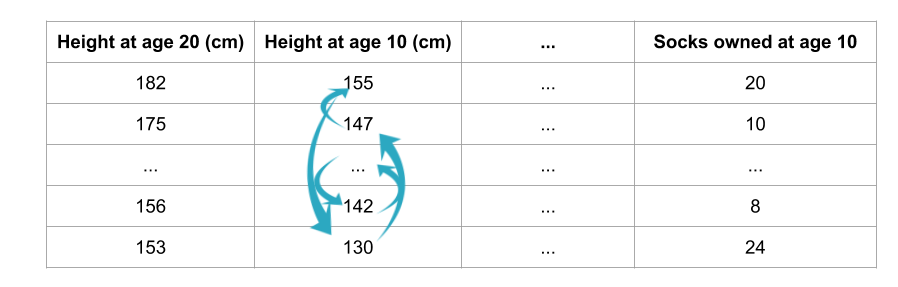
\includegraphics[width=1.\textwidth]{figures/permutation.png}
	\caption{Representation of shuffling the data for a sample data-set. Input values for one features are shuffled randomly switching the data with each other. The score of the model making predictions with these permuted data is computed and compared to the score the model would have for the non-permuted feature.}
	\label{fig:permutation}
\end{figure}

Permutation importance is a simple yet effective way of getting information about which feature drives the outcome in the predictions. 

The data is split into two sub-sets, one for training and one for testing as reported in section \ref{training}. The model is then trained as usual. After training is completed the accuracy of the model is assessed (see Eq. \ref{eq:score}) using the sample left out from the training process. Then the input values from one of the features is randomly shuffled (see, Fig. \ref{fig:permutation}), the $R^2$ score coefficient is computed again, and the change in $R^2$ coefficient between the shuffled and un-shuffled prediction is calculated. 

In this way, for example, for the selected feature $p$, the $i$-th input value corresponding, to the $i$-th output is switched with the $j$-th input, corresponding to the $j$-th output. To compute the score, the model will get the $j$-th input value for the $i$-th output one and vice-versa. This happens for all the input values for the selected feature. The score of the model is computed, and the process is repeated $m$ times in order to have a distribution of scores with different shuffled samples. An average value for the difference between the score of the non shuffled sample and the shuffled one is computed together with its standard deviation.
The permutation importance coefficient for the feature $p$ is then:

\begin{equation}\label{eq:perm}
P_p = \frac{1}{m}\sum_{k=1}^{m}S^*-{S_{p,k}}
\end{equation} 
where $S^*$ represents the score of the non-shuffled sample, and $S_{p,k}$ the score for the $k$-th sample, where the feature $p$ has been shuffled.
The process is repeated for all the features in the input data, and the permutation importance coefficient is calculated for all of them.

A higher coefficient means that shuffling the input values for the considered feature resulted in a decrease in the performance of the model. The higher the permutation importance coefficient then, the higher should be the importance of the feature for computing the prediction. The value of the $P_p$ can be negative meaning that shuffling the features actually improved the performance of the model and that the feature is probably not influencing the prediction.

\subsection{Partial Dependence Plots}
Partial dependence plots are simple charts, which show the change in value of the prediction, dependent on the change in value for the feature one wants to analyze. Each feature value is changed without changing the others, which allows for a visualization of how each feature partially influences the outcome of the prediction. Features more relevant to the prediction will show larger changes in the prediction outcome.

For the linear regression model these plots will look like straight lines, with steeper lines indicating more relevance in the prediction outcome. For non linear models these lines could diverge very much from a straight line; the feature could be more or less relevant depending on the feature value itself.  

\section{Choosing the Features to train the models}\label{features}

\begin{table}[!bp]
	\centering
	\caption{Representation of the data-set used to train the model: rows are grid cells with thickness observations associated with them. Each row contains $p$ features and a single thickness value.}
	\label{tab:features}
	\begin{tabular}{|c|c|c|c|c|c|c|} 
		\cline{2-7}
		\multicolumn{1}{l|}{} & Feature 1 & ... & Feature $j$ & ... & Feature $p$ & Thickness \\  
		\hline
		$x_1$              & $x_{11}$ & ... & $x_{1j}$     & ... & $x_{1p}$     & $y_1$ \\   
		\hline
		...                   & ...       & ... & ...           & ... & ...           & ...    \\     
		\hline
		$x_i$              & $x_{i1}$ & ... & $x_{ij}$     & ... & $x_{ip}$     & $y_i$    \\
		\hline
		...                   & ...       & ... & ...           & ... & ...           & ...  \\       
		\hline
		$x_n$              & $x_{n1}$ & ... & $x_{nj}$     & ... & $x_{np}$     & $y_n$   \\      
		\hline
	\end{tabular}
\end{table}


The GlaThiDa database comes ``only'' with ice thickness observations. There is no information about relevant data which could influence the ice thickness distribution for the glaciers. To train a machine learning model however, it is necessary to feed the algorithm on some input variables, which should influence the ice thickness. Any variable could be chosen in order to do this, but it is sensible to choose from those, which are believed to be responsible for the ice thickens distribution. At the end of the process of choosing the features we end up with a data-set looking like Table \ref{tab:features}. Each row represents a grid cell of the glacier surface map with ice thickness observations, and each of them is associated with $p$ features. Features are used as input values from the machine learning algorithm, and the ice thickness measurements are the desired output or label, for these input values. 


\subsection{The features chosen}\label{features-chosen}
The input variables used to train the models have been chosen from simple geometrical and physical assumptions. They are:

\begin{itemize}
	\item Topography (Altitude above sea level)
	\item Distance from the border of the glacier
	\item Slope angle
	\item Altitude Dependent Linear Mass Balance 
\end{itemize}
The altitude has been chosen for two reasons: relative altitude, altitude compared to the lowest point of the glacier, is a proxy for glacier flow as the ice-flow in a glaciers is driven by gravity. Absolute altitude, on the other hand, can be useful in determining differences between one glacier and another.

The distance from the border is calculated as the distance to the nearest glacier border. In general, it should be proportional to the ice thickness, as in general the ice gets thinner near the borders of the glaciers and thicker in its center. 

The slope angle determines the steepness of the topography, and is calculated through its gradient. A higher slope angle should correspond to thinner ice thickness \cite[P. 298]{cuffey2010physics}.

The altitude dependent linear mass balance  is a constant mass balance as a linear function of altitude. It assumes that the altitude integrated mass balance over the whole glacier surface is zero. The point-wise altitude dependent linear mass balance for each grid-cell, is computed as the linear mass balance of the grid-cell itself, plus the sum of the of the liner mass balance of all the grid-cells above it. Larger altitude dependent linear mass balance mean that the grid cell is accumulating more ice than it is losing, hence it should mean thicker ice. 
  
\subsection{Obtaining the features values}
As mentioned GlaThiDa comes with no information about the glaciers aside for the ice thickness observations. In order to get the input data mentioned in the previous section, the OGGM model has been used. This is an open source python based model for modeling glaciers around the globe. The main way it has been used for this thesis was to download and put together the digital elevation models, smooth them if needed and project them to create a map of the glaciers using RGI for the glaciers outlines. The features where then computed from OGGM using basic geometrical formulas. 

Each entry point in the training data-sets corresponds then to a grid cell of the DEM created by OGGM. The ice thickness used as label for the training data-sets is then not directly the one coming from the GlaThiDa database. It is rather the averaged ice thickness observed over the grid cell of the DEM.

\subsection{Scaling the Features}
Before training a support vector machine algorithm, it is important to apply scaling to the data fed to the algorithm \citep{ScalingSVM2003}. Scaling in this context means the normalization of the features, before training the model. This is done for two main reasons: to avoid features in greater numeric ranges dominating those in smaller numeric ranges, and to avoid some numerical difficulties during computation. This procedure is not required either for linear regression or for random forest regression. In this work however all the data fed to all the algorithms have been scaled. This should not make the performance of the other algorithms worse, but it allows for an easier comparison between the models, especially when looking at the importance of each features.

The \href{https://scikit-learn.org/stable/modules/generated/sklearn.preprocessing.StandardScaler.html}{sklearn.StandardScaler} class has been used to achieve the scaling. If we call the scaled $p-$th feature $z_{ip}$, the mean for the same feature $\overline{x_p}$ and its standard deviation $\sigma_p$ the formula for scaling each feature becomes:

\begin{equation}\label{eq:scale}
z_{ip} = \frac{(x_{ip} - \overline{x_p})}{\sigma_p}
\end{equation}

This transforms the data such that the mean of the scaled feature is $\overline{z_p}=0$ and its standard deviation $\sigma^z_p=1$.

\subsection{Training Region}\label{alps}
In principle a supervised machine learning algorithm could learn from any input data which has an associated label. As explained in section \ref{glathida-stats}, many glaciers in the GlaThiDa only have very few thickness observations. Extrapolating the thickness distribution for those glaciers from those few observations would be very difficult. These sparse measurements however can still be used well by the machine learning algorithm to train the model. In principle then each observation is a useful one, even if it was the only one available for a single glacier. One could then use all the thickness observations present in the GlaThiDa data-set to train the model. In this way we could potentially train a model, which could predict the ice thickness for glaciers on the whole globe.

As mentioned in section \ref{features-chosen}, the only features chosen for training the algorithm are those related to the geometrical properties of the glacier surface. No other piece of information, such as, for instance, the climate of the glacier region, is used to train the model. This could lead to a model which is not very precise in assessing the ice thickness of the glaciers. Furthermore regions with more thickness observations, would create a bias in training the algorithm. Those regions could end up influencing the model output for the whole globe.

In order to avoid these problems we decided to arbitrarily train all the models on region 11 of the RGI inventory, corresponding to Central Europe and in particular the Alps. This region accounts for a total of 3297 glaciers. Of those glaciers however only 106 have thickness observations in the GlaThiDa. After assigning each of these observations to a grid cell in each glacier map, the total number of thickness measurements available to train the models are 8800. When cross validating the model as described in section \ref{training}, a total of 6600 measurements are then used to train the models and 2200 to test them.

\section{Volume Comparison}
After training the machine learning algorithms with GlaThiDa observations and the features mentioned in section \ref{features-chosen} for glaciers with observations in the Alps, the models have been used to compute the total ice volume of all the glaciers in the Alps. The values obtained by these models are then compared to the ones obtained by \citet{Farinotti2019} who created a database of ice volume values for all the glaciers in the RGI inventory. This was created with an ensemble of 5 physically based glacier models. For the alpine region this include 3927 glaciers. However due to problems with computing some of the features needed to predict ice thickness with the machine learning models, 36 of those glaciers have been left out of the predictions with those models. According to the data from \citet{Farinotti2019} these 36 glaciers account for 0.06\% of the total volume of glaciers in the Alps. For the remaining 3891 glaciers in the alps \citet{Farinotti2019} predict a total volume of $1.29\times 10^{11}m^3$.


\section{Data and code availability}
In this section the source of all the data and code used for this thesis is presented.

\subsection{Data}
\begin{itemize}
	\item GlaThiDa: \href{https://www.gtn-g.ch/data_catalogue_glathida/}{https://www.gtn-g.ch/data\_catalogue\_glathida/}
	\item RGI: \href{https://www.glims.org/RGI/}{https://www.glims.org/RGI/}
	\item SRTM (DEM) \href{http://srtm.csi.cgiar.org/}{http://srtm.csi.cgiar.org/}
	\item Glacier volumes by \citet{Farinotti2019}: \href{https://github.com/OGGM/world-glacier-explorer/tree/master/data}{https://github.com/OGGM/world-glacier-explorer/tree/master/data}
\end{itemize}

Other digital elevation models (DEMs) have been used to generate the statistics about GlaThiDa in section \ref{glathida-stats}.

\subsection{Code}
All the analysis and scripts used for this thesis have been written in python.
\begin{itemize}
	\item Analysis results and discussion: \href{https://github.com/MatCast/GlaThiDa-RGI}{https://github.com/MatCast/GlaThiDa-RGI}
	\item Machine learning resources: \href{https://scikit-learn.org/}{https://scikit-learn.org/}
	\item Creation of features and glaciers grid-maps: \href{https://docs.oggm.org/}{https://docs.oggm.org/}
\end{itemize}


 

%\subsubsection{Subsubsection}
%You can also use ``subsubsections''. However, they do not carry a separate
%heading number and they do not appear in the Table of Contents.

%\subsection{Equation}
%As an example for the \verb|equation| environment, I show the equations used in
%the numerical shallow-water model (SWM) developed by
%\citet{scha93Aag,scha93Bag}:
%% ---- equation 1:
%\begin{equation}
%\frac{D\hat{u}}{D\hat{t}}+\frac{\partial(\hat{h}+\hat{H})}
%                               {\partial\hat{x}}=0,
%\label{2equ:1}
%\end{equation}
%% ---- equation 2:
%\begin{equation}
%\frac{D\hat{v}}{D\hat{t}}+\frac{\partial(\hat{h}+\hat{H})}
%                               {\partial\hat{y}}=0,
%\label{2equ:2}
%\end{equation}
%% ---- equation 3:
%\begin{equation}
%\frac{\partial\hat{H}}{\partial\hat{t}}+\frac{\partial(\hat{u}\hat{H})}
%                                             {\partial\hat{x}}
%                                       +\frac{\partial(\hat{v}\hat{H})}
%                                             {\partial\hat{y}}
%                                                =0,
%\label{2equ:3}
%\end{equation}
%with the non-dimensional variables (henceforth generally labelled with hats)
%$\hat{u}$ and $\hat{v}$ as the two horizontal velocity components, $\hat{H}$ and
%$\hat{h}$ as fluid layer depth and terrain height, respectively,
%$\hat{Z}=\hat{h}+\hat{H}$ as fluid layer height, and $\hat{t}$ as time.
%Equations~(\ref{2equ:1})--(\ref{2equ:3}) are non-dimensionalized with the
%following scales: a typical length $L$ for the horizontal length scale, the
%initial far-upstream depth of the fluid layer $H_{\infty}$ (with $h_{\infty}=0$)
%for the vertical length scale, the phase speed of linear gravity waves
%$\sqrt{g^*H_{\infty}}$ for the velocity scale, and the time scale
%$L/\sqrt{g^*H_{\infty}}$.
